% The mean value theorem: a point c where the tangent (red) is parallel
% to the secant (green) joining (a, f(a)) and (b, f(b)).
% Source: book/tex/calculus/differentiate.tex (§ Mean value theorem).
\documentclass[border=2mm]{standalone}
\usepackage{tikz}
\begin{document}
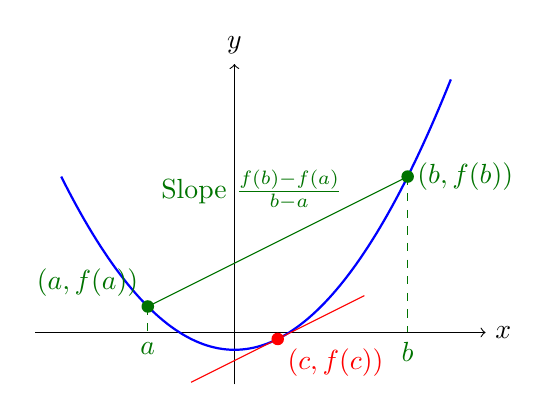
\begin{tikzpicture}[scale=1.1,
    dot/.style={circle,fill,inner sep=1.6pt}]
  \draw[->] (-2.3,0)--(2.9,0) node[right] {$x$};
  \draw[->] (0,-0.6)--(0,3.1) node[above] {$y$};
  \draw[blue,thick,domain=-2:2.5,samples=100]
    plot (\x, {\x*\x/2-0.2});
  % A=(-1,0.3), B=(2,1.8)
  \node[dot,green!45!black] at (-1,0.3) {};
  \node[green!45!black,above left] at (-1,0.3) {$(a,f(a))$};
  \node[dot,green!45!black] at (2,1.8) {};
  \node[green!45!black,right] at (2,1.8) {$(b,f(b))$};
  \draw[green!45!black] (-1,0.3)--(2,1.8);
  \node[green!45!black,above] at (0.2,1.3)
    {Slope $\frac{f(b)-f(a)}{b-a}$};
  \draw[green!45!black,dashed] (-1,0.3)--(-1,0);
  \draw[green!45!black,dashed] (2,1.8)--(2,0);
  \node[green!45!black,below] at (-1,0) {$a$};
  \node[green!45!black,below] at (2,0) {$b$};
  % c = 0.5, f(c) = -0.075; tangent slope 0.5
  \node[dot,red] at (0.5,-0.075) {};
  \node[red,below right] at (0.5,-0.075) {$(c,f(c))$};
  \draw[red] (-0.5,-0.575)--(1.5,0.425);
\end{tikzpicture}
\end{document}
